% !TEX TS-program = XeLaTeX
% use the following command:
% all document files must be coded in UTF-8
\documentclass[spanish]{textolivre}
% build HTML with: make4ht -e build.lua -c textolivre.cfg -x -u article "fn-in,svg,pic-align"

\journalname{Texto Livre}
\thevolume{16}
%\thenumber{1} % old template
\theyear{2023}
\receiveddate{\DTMdisplaydate{2023}{5}{23}{-1}} % YYYY MM DD
\accepteddate{\DTMdisplaydate{2023}{8}{20}{-1}}
\publisheddate{\DTMdisplaydate{2023}{11}{5}{-1}}
\corrauthor{Arturo Amaya Amaya}
\articledoi{10.1590/1983-3652.2023.46297}
%\articleid{NNNN} % if the article ID is not the last 5 numbers of its DOI, provide it using \articleid{} commmand 
% list of available sesscions in the journal: articles, dossier, reports, essays, reviews, interviews, editorial
\articlesessionname{articles}
\runningauthor{García Mercado et al.} 
%\editorname{Leonardo Araújo} % old template
\sectioneditorname{Hugo Heredia Ponce}
\layouteditorname{Thaís Coutinho}

\title{Mediaa Music, innovando método de enseñanza/aprendizaje del idioma inglés a través de canciones}
\othertitle{Mediaa Music, inovando o método de ensino/aprendizagem da língua inglesa através de músicas}
\othertitle{Mediaa Music, innovating the teaching/learning method of the English language through songs}
% if there is a third language title, add here:
%\othertitle{Artikelvorlage zur Einreichung beim Texto Livre Journal}

\author[1]{Daniel García Mercado~\orcid{0000-0002-7041-3367}\thanks{Email: \href{mailto:daniel.garcia@utmatamoros.edu.mx}{daniel.garcia@utmatamoros.edu.mx}}}
\author[2]{Arturo Amaya Amaya~\orcid{0000-0002-6614-4256}\thanks{Email: \href{mailto:arturo.amaya@docentes.uat.edu.mx}{arturo.amaya@docentes.uat.edu.mx}}}
\author[1]{Daniel Cantú Cervantes~\orcid{0000-0001-8652-3707}\thanks{Email: \href{mailto:dcantu@docentes.uat.edu.mx}{dcantu@docentes.uat.edu.mx}}}
\affil[1]{Universidad Tecnológica de Matamoros, México.}
\affil[2]{Universidad Autónoma de Tamaulipas, México.}

\addbibresource{article.bib}
% use biber instead of bibtex
% $ biber article

% used to create dummy text for the template file
\definecolor{dark-gray}{gray}{0.35} % color used to display dummy texts
\usepackage{lipsum}
\SetLipsumParListSurrounders{\colorlet{oldcolor}{.}\color{dark-gray}}{\color{oldcolor}}

% used here only to provide the XeLaTeX and BibTeX logos
\usepackage{hologo}

% if you use multirows in a table, include the multirow package
\usepackage{multirow}

% provides sidewaysfigure environment
\usepackage{rotating}

% CUSTOM EPIGRAPH - BEGIN 
%%% https://tex.stackexchange.com/questions/193178/specific-epigraph-style
\usepackage{epigraph}
\renewcommand\textflush{flushright}
\makeatletter
\newlength\epitextskip
\pretocmd{\@epitext}{\em}{}{}
\apptocmd{\@epitext}{\em}{}{}
\patchcmd{\epigraph}{\@epitext{#1}\\}{\@epitext{#1}\\[\epitextskip]}{}{}
\makeatother
\setlength\epigraphrule{0pt}
\setlength\epitextskip{0.5ex}
\setlength\epigraphwidth{.7\textwidth}
% CUSTOM EPIGRAPH - END

% LANGUAGE - BEGIN
% ARABIC
% for languages that use special fonts, you must provide the typeface that will be used
% \setotherlanguage{arabic}
% \newfontfamily\arabicfont[Script=Arabic]{Amiri}
% \newfontfamily\arabicfontsf[Script=Arabic]{Amiri}
% \newfontfamily\arabicfonttt[Script=Arabic]{Amiri}
%
% in the article, to add arabic text use: \textlang{arabic}{ ... }
%
% RUSSIAN
% for russian text we also need to define fonts with support for Cyrillic script
% \usepackage{fontspec}
% \setotherlanguage{russian}
% \newfontfamily\cyrillicfont{Times New Roman}
% \newfontfamily\cyrillicfontsf{Times New Roman}[Script=Cyrillic]
% \newfontfamily\cyrillicfonttt{Times New Roman}[Script=Cyrillic]
%
% in the text use \begin{russian} ... \end{russian}
% LANGUAGE - END

% EMOJIS - BEGIN
% to use emoticons in your manuscript
% https://stackoverflow.com/questions/190145/how-to-insert-emoticons-in-latex/57076064
% using font Symbola, which has full support
% the font may be downloaded at:
% https://dn-works.com/ufas/
% add to preamble:
% \newfontfamily\Symbola{Symbola}
% in the text use:
% {\Symbola }
% EMOJIS - END

% LABEL REFERENCE TO DESCRIPTIVE LIST - BEGIN
% reference itens in a descriptive list using their labels instead of numbers
% insert the code below in the preambule:
%\makeatletter
%\let\orgdescriptionlabel\descriptionlabel
%\renewcommand*{\descriptionlabel}[1]{%
%  \let\orglabel\label
%  \let\label\@gobble
%  \phantomsection
%  \edef\@currentlabel{#1\unskip}%
%  \let\label\orglabel
%  \orgdescriptionlabel{#1}%
%}
%\makeatother
%
% in your document, use as illustraded here:
%\begin{description}
%  \item[first\label{itm1}] this is only an example;
%  % ...  add more items
%\end{description}
% LABEL REFERENCE TO DESCRIPTIVE LIST - END


% add line numbers for submission
%\usepackage{lineno}
%\linenumbers

\begin{document}
\maketitle

\begin{polyabstract}
\begin{abstract}
El objetivo de esta investigación fue identificar si un método didáctico basado en canciones originales en inglés denominado Mediaa Music puede favorecer el aprendizaje del idioma de los alumnos de educación superior ($n=80$) en los niveles A1 y A2 con base en el MCER, en dos universidades en México durante 2021. Mediante un enfoque cuantitativo con diseño cuasiexperimental y alcance descriptivo, se logró identificar que el grupo de intervención (Hombres: $n=20$, Edad: $M=19.84$, DE $\pm 0.824$, $\text{Max}=20$, $\text{Min}=18$; Mujeres: $n=20$, Edad: $M=20.43$, DE $\pm 0.184$, $\text{Max}=21$, $Min=18$) mostró puntajes con diferencias significativas ($p<.05$) al ser expuestos a la propuesta de Mediaa Music en comparación con el grupo control (Hombres: $n=20$, Edad: $M=20.16$, DE $\pm 1.884$, $Max=20$, $Min=18$; Mujeres: $n=20$, Edad: $M=20.80$, DE $\pm 1.825$, $\text{Max}=20$, $\text{Min}=18$) que estudiaron solo con textos escritos. No se identificaron diferencias significativas ($p>.05$) de tendencia central entre los puntajes obtenidos por los alumnos de ambas instituciones, ni en el género de los participantes.

\keywords{Inglés \sep Aprendizaje \sep Enseñanza Superior \sep Música}
\end{abstract}

\begin{portuguese}
\begin{abstract}
O objetivo desta pesquisa foi identificar se um método de ensino baseado em músicas originais em inglês, chamado Mediaa Music, pode promover a aprendizagem de línguas de estudantes do ensino superior ($n=$80) em duas universidades no México durante 2021. Por meio de uma abordagem quantitativa com desenho quase experimental e escopo descritivo, foi possível identificar que o grupo de intervenção (Homens: $n=20$, Idade: $M=19,84$, DP $\pm 0,824 $, $\text{Max}=20$, $\text{Min}=18$; Mulheres: $n=20$, Idade: $M=20,43$, SD $\pm 0,184$, $\text{Max}=21$, $Min=18$) apresentaram pontuações com diferenças significativas ($p<0,05$) quando expostos à proposta da Mediaa Music em comparação ao grupo controle (Homens: $n=20$, Idade: $M= 20,16$, SD $\pm 1,884$, $Max=20$, $Min=18$; Mulheres: $n=20$, Idade: $M=20,80$, SD $\pm 1,825$, $\ text{Max }=20$, $\text{Min}=18$) que estudaram apenas com textos escritos. Não foram identificadas diferenças significativas ($p>0,05$) de tendência central entre as pontuações obtidas pelos alunos das duas instituições, nem no sexo dos participantes.

\keywords{Inglês \sep Aprendizagem \sep Ensino Superior \sep Música}
\end{abstract}
\end{portuguese}

\begin{english}
\begin{abstract}
This research aimed to identify if a didactic method based on original songs in English called Mediaa Music can improve the learning of the language of higher education students ($n=80$), in two universities in Mexico in 2021. Through a quantitative approach with design quasiexperimental and descriptive scope, it was possible to identify that the intervention group (Men: $n=20$, Age: $M=19.84$, SD $\pm 0.824$, $\text{Max}=20$, $\text{Min}=18$; Women: $n=20$, Age: $M=20.43$, SD $\pm 0.184$, $\text{Max}=21$, $\text{Min}=18$) showed scores with significant differences ($p<.05$) when exposed to the Mediaa Music proposal compared to the control group (Men: $n=20$, Age: $M=20.16$, SD $\pm 1.884$, $\text{Max}=20$, $\text{Min}=18$; Women: $n=20$, Age: $M=20.80$, SD $\pm 1.825$, $\text{Max}=20$, $\text{Min}=18$) who
studied only with written texts. No significant differences ($p>.05$) in central tendency were identified between the scores obtained by the students of both institutions, neither in the gender of the participants.

\keywords{English \sep Learning \sep Higher Education \sep Music}
\end{abstract}
\end{english}
% if there is another abstract, insert it here using the same scheme
\end{polyabstract}

\section{Introducción}

La música es un estímulo psicobiológico sensorial, cognitivo y motor que consiste en estructuras de sonidos organizados en el tiempo que promueven imaginerías mentales episódicas e inefables que se crean de acuerdo con la experiencia de cada persona \cite{talamini2018learning}. La comprensión musical requiere de la decodificación de patrones acústicos sobre las relaciones de sonidos consecutivos bajo la intensidad y frecuencia de cadencias tonales armónicas y melódicas de la pieza \cite{matute2012tendencias}, que estimulan al oyente y le generan significados emocionales \cite{khan2018effects}.

La música impacta de manera favorecedora el aprendizaje de los idiomas cuando la lírica se encuentra directamente relacionada con los contenidos a aprender \cite{widerman2013study, harding2019cortical}, por ejemplo, cuando se armoniza con movimientos \emph{ad hoc}, como ademanes y cuando el contenido musical es puntual para la tarea que se va a aprender \cite{galinska2015music, biasutti2019self}. Además, las piezas musicales preferidas por el sujeto aumentan la motivación de este, facilitan la relajación vascular y disminuyen el estrés \cite{mcclurkin2016duration}. 

Diversas investigaciones realizadas por \textcite{skeja2014impact}, \textcite{hafting2018benefits}, \textcite{azaryahu2020musimath} y \textcite{hakvoort2022music}, han señalado que los programas de intervención con piezas musicales alineados a los ejes temáticos muestran mejoras significativas que otros programas musicales ajenos a los contenidos. Esto debido a que se ha identificado según \textcite{perham2011can} y \textcite{penagos2012efectos}, que las piezas musicales aumentan una respuesta emocional más alta en el oyente que en condiciones de silencio. En este sentido, se ha sugerido por parte de \textcite{damasio2000feeling}, \textcite{manes2014usar}, \textcite{kyriazi2018}, que las emociones favorecen la vividez de las unidades mentales de significado, favoreciendo recuerdos más perdurables.

El aprendizaje del idioma inglés se ha estandarizado en el mundo escolarizado \cite{legacy2017dog}, debido a su impacto socio comercial, académico, científico y tecnológico \cite{delos2020grammatical}. El aprendizaje de los idiomas se ha vuelto una competencia estándar para los profesionistas debido al alcance social y productivo que genera el comprender más de una lengua \cite{vagh2009measuring}. No solo la globalización del mercado ha fomentado el plurilingüismo, sino la globalización de la información que acerca a sus consumidores al aprendizaje de lenguajes comunes en el mundo, para acceder a mayor cantidad de contenido y de relaciones productivas, académicas y científicas \cite{core2013total}. Por otra parte, se ha destacado que el conocimiento de idiomas aumenta hasta un 37\% las posibilidades de acceder a un empleo, siendo esta capacidad la que más incrementa las expectativas de los profesionales para emplearse, principalmente porque el 26\% de las ofertas actuales en el mercado laboral exige conocimiento de algún idioma extranjero, siendo el inglés el más demandado \cite{randstad2017}.

La pedagogía de los idiomas como ciencia progresiva premia los esfuerzos constantes de las instituciones y de los docentes por mejorar las prácticas educativas en el aprendizaje de las lenguas, en el caso de México, del idioma inglés \cite{legacy2017dog}. Los esfuerzos institucionales no se han agotado en el sentido de favorecer el desarrollo de propuestas eficaces que motiven el desarrollo de mejores aprendizajes específicos del idioma para beneficiar a sus estudiantes \cite{vagh2009measuring}. El uso de la música (con lírica relacionada con el contenido) en el aprendizaje, no es un tema novedoso en el campo, de manera que diversos estudios como los de \textcite{moradi2014effect}, \cite{shehadejiman2016effectiveness}, \textcite{yusmita2017effects}, \cite{suwartono2019songs}, \cite{jabak2021role}, \textcite{saldiraner2021using} y \textcite{hakvoort2022music}, han mostrado que puede favorecer la aprehensión del idioma inglés en aprendices escolarizados.

La comprensión del idioma inglés requiere el desarrollo de habilidades como la dicción, pronunciación y comprensión, los cuales se rodean de distintas reglas gramaticales necesarias \cite{rauscher2016music}. La adquisición de estas habilidades se facilita con la presencia de música, propiciada a través de la rima, la melodía y el canto \cite{kafol2015analysis}, que disminuyen el aburrimiento, aumentan la repetición de los ejercicios y ayudan en la memorización del vocabulario, la pronunciación y la gramática \cite{shehadejiman2016effectiveness}. De forma contemporánea, los maestros han usado la técnica de las canciones para impulsar los aprendizajes de idiomas por la respuesta emocional que evocan y la motivación que generan en los aprendices \cite{brown2010arts}.

Las canciones modernas populares se han distinguido por contener acordes melódicos simples y repetitivos, ya que se vuelven fáciles para la percepción armónica del promedio de las personas según \textcite{chiang2018language}, especialmente por los no músicos \cite{harding2019cortical}(. Además, suelen incorporar prosa con semántica sencilla con tintes sentimentales y emocionales que se relacionan con la experiencia común de las personas \cite{talamini2018learning}. Esto permite que la mayor parte de los usuarios puedan comprender las cadencias musicales y sus líricas, haciendo populares a dichas piezas musicales \cite{kim2014melody}.

Se ha identificado que melodías con cadencias tonales mayores generalmente promueven respuestas perceptivas alegres, mientras que las cadencias en tonos menores se relacionan con respuestas más melancólicas \cite{jancke2010music, hallam2010effects}. Cuando una cadencia posee múltiples variaciones armónicas, las personas no músicos pueden encontrar más difícil comprender o predecir las melodías, que cuando las cadencias son simples y repetitivas \cite{zhang_background_2014, chiang2018language}. Además, cuando el ritmo es rápido las respuestas vasculares aumentan, y cuando es lento tienden a disminuir \cite{aljanaki2016studying}.

\section{Antecedentes}

\textcite{saldiraner2021using}, implementaron un programa de intervención con canciones para aprender inglés en estudiantes ($n=72$) de secundaria, mediante un estudio experimental donde el grupo control recibió solo textos con actividades escritas. Ambos grupos fueron evaluados previo y posterior a la intervención, y mediante un análisis de varianza, los resultados mostraron que los puntajes del grupo experimental fueron mayores con diferencias significativas respecto al grupo de comparación según datos similares reportados por \textcite{forster2006value}.

Por otra parte, \textcite{ghanbari2014effects}, trabajaron con 60 estudiantes de educación primaria, mediante un programa de intervención de canciones con contenidos temáticos de inglés en dos grupos de comparación. Mediante pruebas de varianza de diferencias de medias, identificaron un efecto positivo en el grupo experimental respecto al grupo de control sin diferencias significativas entre el género de los participantes. Hallazgos similares también han sido reportados por \textcite{kocaman2016effects} y \textcite{wahyuningsih2019kreasi}.

Por otro lado, \textcite{moradi2014effect}, implementaron un programa de canciones para aprender inglés a una muestra de 30 estudiantes de educación primaria con el fin de que los alumnos las repitieran y las memorizaran. El grupo control estudió las canciones sin la intervención de la música. Los resultados pretest y postest mediante un análisis t (muestras independientes) revelaron que el grupo experimental mostró mayores puntajes que el grupo de comparación con diferencias significativas de medias aritméticas (datos similares reportados por \textcite{lestari2020vocabulary}).

Por otra parte, \textcite{shehadejiman2016effectiveness}, identificaron mayores puntajes con diferencias significativas (análisis t de muestras independientes) en alumnos ($n=58$) que estudiaron con ayuda de canciones para aprender inglés en comparación con estudiantes ($n=65$) del grupo de comparación. Los hallazgos además indicaron que los docentes consideran a las canciones como herramientas didácticas valiosas para aprender inglés, por ser contenidos que precisan de la praxis como eje principal \cite{shehadejiman2016effectiveness}. Estos datos son semejantes a los reportados por \textcite{yusmita2017effects}, quienes identificaron mediante un análisis t, puntajes superiores con diferencias significativas en alumnos que estudiaron usando canciones para aprender inglés, que alumnos que estudiaron los mismos contenidos en materiales escritos.

Por otro lado y bajo un enfoque mixto, \textcite{ratnasari2007}, identificó que las canciones para aprender inglés mejoraron el aprendizaje de la lengua tanto en vocabulario, gramática y pronunciación en estudiantes ($n=30$) de séptimo grado de escuela elemental. Aunque en este estudio no se aplicaron análisis paramétricos inferenciales, se logró apreciar un progreso en los promedios alcanzados por los alumnos tratados con la variable independiente. Datos similares reportados por \textcite{shen2009using} y \textcite{farmand12013effect}.

Entre estudios de corte experimental, se distinguen \textcite{suwartono2019songs}, quienes reportaron mejoras en los aprendices que estudiaron con canciones para aprender inglés, no obstante, las pruebas de diferencias de medias (t para muestras independientes) no reportaron diferencias significativas entre el grupo con tratamiento y el control (datos similares reportados por \textcite{jabak2021role}). Otros hallazgos son los reportados por \textcite{javadisafa2018effects}, quien identificó bajo un análisis t, mejoras significativas en el grupo que estudió con canciones en inglés para aprender vocabulario, respecto al grupo de comparación que estudió los mismos contenidos en prosa sin presencia de música. Otros hallazgos similares fueron reportados por \textcite{komur2005teaching}, \textcite{malekian2016relationship}, \textcite{andradesanchez2017use} y \textcite{luo2019influence}.

La mayor parte de los estudios de intervención con canciones para aprender inglés que realizaron \textcite{komur2005teaching}, \textcite{forster2006value}, \textcite{ghanbari2014effects}, \textcite{moradi2014effect}, \textcite{malekian2016relationship}, \textcite{javadisafa2018effects}, \textcite{wahyuningsih2019kreasi}, \textcite{suwartono2019songs}, \textcite{jabak2021role} y \textcite{saldiraner2021using}, no usaron canciones inéditas en el tratamiento de la variable independente, sino piezas musicales ya elaboradas; además, se enfocaron en analizar la significancia de diferencias de medias aritméticas en pruebas con muestras independentes sin considerar pruebas post hoc con tamaños del efecto y potencia estadística. Por otro lado, gran parte de las intervenciones realizadas por \textcite{farmand12013effect}, \textcite{ghanbari2014effects}, \textcite{shehadejiman2016effectiveness}, \textcite{malekian2016relationship}, \textcite{manikandan2011frequency}, \textcite{javadisafa2018effects}, \textcite{suwartono2019songs} y \textcite{saldiraner2021using}, utilizaron los materiales de libro de texto institucionales de la asignatura de inglés para medir los resultados.

\textcite{lestari2020vocabulary}, indican que un repertorio de canciones originales puede ser más flexible para adaptarse al contexto de estudio respecto a los aprendizajes esperados, porque como señalan \textcite{hafting2018benefits} y \textcite{hakvoort2022music}, cuanto más puntual sea la canción respecto al objetivo de estudio, más probabilidades se generan para encontrar mejores resultados. La dificultad de esta tarea sin embargo, es la pericia musical que requiere la producción musical y la didáctica de las líricas para mejorar el aprendizaje adaptativo mediante canciones originales.

Como antesala de esta investigación, hasta el momento no se han reportado estudios de intervención en las Instituciones de Educación Superior en México que hayan utilizado métodos didácticos basados en canciones elaboradas originales e inéditas que promuevan el aprendizaje específico del idioma inglés. Con base en lo anterior, surge el interés de dar respuesta a la siguiente pregunta de investigación:

\begin{quote}
 ¿Cuáles son las diferencias entre alumnos de educación superior que apoyaron su aprendizaje del idioma inglés a través del método Mediaa Music y alumnos que utilizaron el método didáctico tradicional, basado en textos escritos?
\end{quote}

En este procedimiento se estableció el objetivo de identificar si un método didáctico basado en canciones originales en inglés puede favorecer el aprendizaje del idioma de alumnos de educación superior en los niveles A1 y A2 con base en el MCER, en dos universidades de México.





\section{Método MEDIAA MUSIC}

\textcite{ledezmaalbarran2013estudios}, indica que los programas de intervención en estudios cuasiexperimentales se distinguen por ser propuestas de desarrollo basadas en literatura preexistente que tienen en lo general como objetivo mejorar una condición determinada. La propuesta Mediaa Music es una iniciativa inédita que comprende una librería de cuatro canciones originales para aprender inglés, para el marco gramatical del verbo “To Be”, se utilizó la canción “We Are”; para el “Presente Simple”, se utilizó “Party”; para el “Pasado Simple”, se utilizó “What Did I Get”; y para el “Presente Perfecto”, se utilizó “Have You Ever Missed Me”, es decir, una canción para cada tema. Las canciones han sido compuestas de manera básica en su estructura musical para fungir como el canal para la transmisión del mensaje o letra que aborde desde su estructura general un tema gramatical en específico, logrando tener coherencia y sentido en su historia y redacción... La originalidad del contenido de la propuesta favorecerá la no violación de derechos de autor, así como la flexibilidad de adaptación a los contenidos impartidos \cite{lestari2020vocabulary}.

La estructura lírica se apegó a la forma base (estrofa, estribillo, estrofa, estribillo) con una duración aproximada de 3 minutos por canción \cite{martinez2017}. El género musical se definió con base en los tres grandes géneros comerciales y populares actuales (pop, balada y urbano) \cite{sinaga2019learning}, y se persiguió la progresión de acordes simple (grados I-V-VI-IV) más usada en géneros como el pop y el rock \cite{martinez2017}, por su sencillez iterativa y versatilidad de orden \cite{kim2014melody}. La sencillez y uso de rimas en las canciones, el estilo de género similar al comercial y la progresión de acordes simple, podrían mejorar la comprensión melódica de la mayoría de los estudiantes, especialmente en aquellos que no son músicos \cite{chiang2018language}.

En la \Cref{fig1} se presenta el proceso y puntos clave de producción lírica, donde la producción lírica se divide en seis pasos: Gramática, que es la elección del tema gramatical a abordar en la canción inédita; Vocabulario, que es la elección de vocabulario de acuerdo con el MCERL y tema gramatical; Temática, que es la elección de temática de la canción: balada, pop, rock, urbano, fusiones e historia; Desarrollo de la historia de la canción: amor, desamor, aventura, entre otras; Trama, que es el desarrollo de la trama: personajes, tiempos, secuencias, situaciones; y Letra, que es el desarrollo a formato de canción estructurando estrofas, estribillos, pre-coro, coros, con sus respectivas rimas y versos.

\begin{figure}[h!]
\centering
\begin{minipage}{.8\textwidth}
 
\includegraphics[width=\textwidth]{image1.jpg}
 \caption{Proceso de producción lírica.}
 \label{fig1}
 \source{Elaboración propia.}
\end{minipage}
\end{figure}

En la \Cref{fig2} se presenta el proceso y puntos clave de producción musical, la cual se divide en seis pasos: Planeación de los tiempos, etapas, contenido, locaciones y detalles de la producción entre productor musical y coordinador de inglés; Preproducción se refiere a la composición de la producción musical definiendo género y progresiones rítmicas, armónicas y melódicas, además de detalles de sonido y músicos participantes por parte del productor/director musical; Grabación de instrumentación vía controladores y/o MIDI para la realización de pistas realizado por el productor/director musical, o grabación de pista musical con músicos de estudio por parte del equipo de músicos e intérpretes vocales; Postproducción, que corresponde a la mezcla, edición, masterización, toques y detalles de sonido y realizados por el ingeniero de grabación; Distribución, que se refiere al almacenamiento en catálogo de MEDIAA Music y en plataformas digitales que promuevan la interacción, facilidad y usabilidad con el usuario; y Aplicación, que es la interacción y aplicación de determinada canción de MEDIAA Music y usuario, según lo estipulado por las indicaciones del profesor e instrucciones de uso dentro y fuera del aula.

\begin{figure}[h!]
\centering
\begin{minipage}{.8\textwidth}
 
\includegraphics[width=\textwidth]{image2.png}
 \caption{Proceso de producción musical.}
 \label{fig2}
 \source{Elaboración propia.}
\end{minipage}
\end{figure}

Es importante mencionar que la producción lírica y musical de las piezas musicales fue supervisada por DGM (autor) a través de un teclado SRK MIDI keyboard controler, que es un controlador de 37 teclas con conexión de entrada y salida MIDI, USB sencilla y de simple configuración. El control de edición (cortes, efectos) y masterización (comprensión, normalización) de producción se realizó mediante el software Garage Band (Logic Pro) para el sistema operativo Macintosh, con soporte de dos altavoces profesionales de dos vías modelo JBL 306P MkII de 6 pulgadas. La captación de voz y coros se llevó a cabo mediante el micrófono condensador profesional de estudio modelo Neewer NW-800. El formato de salida de comprensión se estableció en MP3 (Mpeg Audio Layer III) por ser un código de reproducción común para los dispositivos reproductores de audio \cite{sinaga2019learning}. Las canciones masterizadas se colocaron en una dirección web de almacenamiento con acceso abierto. El proceso de producción se adecúo con base en metodologías de expertos, en el área de la didáctica musical y en el área de la instrucción de la lengua inglesa \cite{linares2018elaboracion}.

Para realizar los procesos de producción lírica y musical, fue necesario conformar un equipo de expertos en la materia. En la \Cref{fig3} se menciona cada uno de ellos, así como sus funciones en esta investigación, donde el equipo de la producción lírica, fueron los responsables de la creación del contenido lírico de la canción a componer, y se integró por expertos en el idioma inglés y en creatividad artística con un enfoque en composición de canciones; y el equipo de la producción musical, se integró principalmente de músicos lidereados por un productor y director musical, quienes elaboraron la canción desde una perspectiva musical, basándose en la información lírica y acotada al grupo de inglés.

\begin{figure}[h!]
\centering
\begin{minipage}{.8\textwidth}
 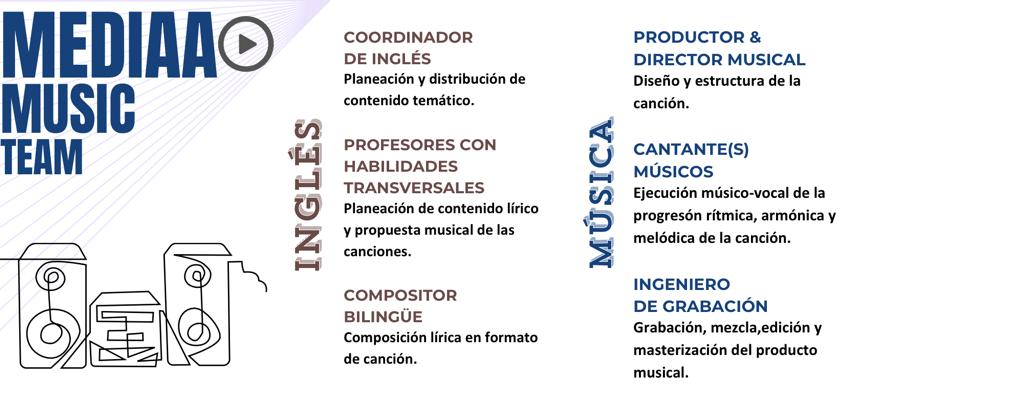
\includegraphics[width=\textwidth]{image3.jpeg}
 \caption{Equipo Mediaa Music.}
 \label{fig3}
 \source{Elaboración propia.}
\end{minipage}
\end{figure}



\section{Metodología}

Esta investigación es de corte cuasiexperimental descriptiva con base en sus objetivos y cuantitativa por su enfoque analítico y tipo de datos usados \cite{hernandez2014metodologia}. El objetivo fue identificar si un método didáctico basado en canciones originales en inglés puede favorecer el aprendizaje del idioma de los alumnos de educación superior en los niveles A1 y A2 con base en el MCER, en dos universidades de México. Los datos se recopilaron durante 2021 donde se trabajó con un total de 80 estudiantes de educación superior de la Universidad Autónoma de Tamaulipas (UAT) ($n=40$) y de la Universidad Autónoma del Noreste (UANE) ($n=40$) ubicadas en Cd. Matamoros, Tamaulipas, México. La factibilidad del presente estudio se logró por la facilidad de los investigadores para trabajar con dicha población. Se establecieron las siguientes hipótesis direccionales:

\begin{description}
\item[$H_1$]: los participantes de la UAT y UANE muestran diferencias significativas entre sí en los puntajes obtenidos.
\item[$H_0$]: los participantes de la UAT y UANE no muestran diferencias significativas entré sí en los puntajes obtenidos.
\item[$H_2$]: los participantes de ambos grupos de comparación difieren significativamente en sus puntajes obtenidos.
\item[$H_0 2$] los participantes de ambos grupos de comparación no difieren significativamente en sus puntajes obtenidos.
\item[$H_3$]: el género de los participantes muestra diferencias significativas entré sí respecto a los puntajes obtenidos.
\item[$H_0 3$]: el género de los participantes no muestra diferencias significativas entré sí respecto a los puntajes obtenidos.
\end{description}



\subsection{Participantes}

Se trabajó con una muestra intencional no probabilística con grupos establecidos de estudiantes ($n=80$, Edad, $M=20.19$, DS $\pm 1.519$, $\text{Max}=21$, $\text{Min}=18$), de los cuales el 50\% ($n=40$) pertenecen a la Universidad Autónoma de Tamaulipas (Edad: $M=19.53$, DS $\pm 0.539$, $\text{Max}=20$, $\text{Min}=18$) y 50\% ($n=40$) a la Universidad Autónoma del Noreste (Edad: $M=20.68$, DS $\pm 1.213$, $\text{Max}=21$, $\text{Min}=18$). Esta población se dividió en dos grupos de comparación con participantes equivalentes: grupo experimental (varones: $n=20$, Edad: $M=19.84$, DS $\pm 0.824$, $\text{Max}=20$, $\text{Min}=18$. Mujeres: $n=20$, Edad: $M=20.43$, DS $\pm 0.184$, $\text{Max}=21$, $\text{Min}=18$) y grupo de control (varones: $n=20$, Edad: $M=20.16$, DS $\pm 1.884$, $\text{Max}=20$, $\text{Min}=18$. Mujeres: $n=20$, Edad: $M=20.80$, DS $\pm 1.825$, $\text{Max}=20$, $\text{Min}=18$). Los grupos de estudio fueron conformados de manera equitativa y equilibrada por un número de integrantes con una competencia idiomática para recibir y producir el idioma extranjero de manera básica a elemental dentro de los niveles A1 y A2, con características similares en conocimiento y habilidades del idioma, según los resultados arrojados por el examen de diagnóstico que se aplicó en ambas instituciones de nivel superior. Es importante mencionar que al ingresar a sus aulas para definir la distribución adecuada de los alumnos en los diferentes niveles de inglés se contó con instrumentos de evaluación con base en metodologías apegadas al MCER, abarcando desde los niveles A1 hasta B2, siendo este último, la meta a alcanzar por el cuerpo estudiantil y definidos como requerimientos de las instituciones de nivel superior.

Durante la aplicación de la variable independiente, no se produjeron abandonos por parte de los participantes. Se siguieron las recomendaciones de investigación establecidas por el Código de Ética de la Universidad Autónoma de Tamaulipas \cite{universida2018}, de tal forma que todos los participantes fueron informados sobre el propósito del estudio y firmaron un consentimiento escrito. Se garantizó la confidencialidad de sus datos personales con fines estrictamente académicos.

Todos los sujetos muestrales manifestaron su voluntad de informar y participar para los fines de esta investigación, pudiendo en cualquier instante abandonar el estudio. No se incentivó a los estudiantes con ningún tipo de estímulo académico o económico con el fin de sesgar su participación o respuestas. Todos los datos recopilados fueron de carácter anónimo que prescindieron de informaciones sensibles y personales como nombres propios y datos de contacto (teléfonos, correos, direcciones, entre otras).


\subsection{Instrumentos}

Se usaron los libros de trabajo del programa de la asignatura de inglés de ambas instituciones. El material usado fue la serie “Going Live” del libro del estudiante de la editorial Edelvives, de Robin y Najma (2015), basado en el nivel A1 y A2 del Marco Común Europeo de Referencia para las Lenguas (2001). La metodología que establece el material es específica con las dimensiones didácticas del aprendizaje de las estructuras del verbo to be, presente simple, pasado simple y perfecto. Las características pedagógicas de estos niveles de acuerdo con el \textcite{mcerl2001}, se implican en el desarrollo de expresiones básicas y necesidades concretas, así como la formulación de preguntas personales y descripción de pertenencias. Por otro lado, premian la repetición de ejercicios con expresiones simples y cotidianas, a la vez que implica al estudiante en la formulación descriptiva del presente simple, pasado simple y pasado perfecto.

Se utilizaron las actividades de evaluación propuestas en el material de trabajo para mesurar el desarrollo de la estructura del verbo to be, el presente simple, pasado simple y pasado perfecto. El libro de actividades posee dos evaluaciones semejantes (diagnóstico y sumativa) distribuidas en 60 reactivos que mesuran los temas (verbo to be, el presente simple, pasado simple y pasado perfecto) a través de ejercicios de competencia lectora (Reading, 10 reactivos), escritura (Writing, 4 reactivos), comprensión auditiva (Listening, 20 reactivos) y reconocimiento Gramatical (26 reactivos) Marco Común Europeo de Referencia para las Lenguas (2001). Cada reactivo tiene valor de un punto sumando un puntaje máximo de 60. La prueba de diagnóstico permitió identificar el puntaje de los participantes previo a la intervención (propuesta del método Mediaa Music), mientras que la prueba sumativa los puntajes posteriores. A continuación, se presenta el procedimiento del trabajo.


\subsection{Procedimiento}

Después de una revisión literaria sobre los antecedentes primarios relacionados con el objeto de estudio y la previa autorización de las autoridades institucionales como lo recomienda Gallardo-Echenique (2017), se aplicó el pretest a los estudiantes ($n=80$) de ambos grupos de comparación, y se implementó la variable independiente al grupo experimental con ausencia de estímulo al grupo de comparación. Se trabajó con ambos grupos con 4 sesiones semanales con duraciones de 60 minutos con los temas del marco gramatical del verbo to be, el presente simple, el pasado simple y el presente perfecto de los contenidos del libro de texto de la asignatura de inglés Student Book “Going Live”, de Editorial Edelvives de \textcite{robin2015}, basado en el Marco Común Europeo de Referencia para las \textcite{mcerl2001}. El tiempo de trabajo no pudo extenderse debido a las limitaciones de agenda de las instituciones participantes. Se les pidió a los estudiantes que recibieron el tratamiento con la propuesta Mediaa Music que escucharan las piezas musicales para fortalecer tanto las habilidades receptoras como las habilidades auditivas, y al paso de horas de exposición, incrementar el enfoque hacia el desarrollo de las habilidades lectoras dentro del aula de clase, con apoyo de las líricas de las mismas canciones expuestas y con ello, provocar la producción del idioma mediante la creación de nuevas propuestas mediante las habilidades escritas y orales bajo la asesoría y guía del docente durante las sesiones destinadas para este ejercicio, partiendo de un contenido preestablecido y enfocado a un tema en específico y llevándolo al aprendizaje adaptativo de los alumnos durante las sesiones de clases.

Por otro lado, los alumnos del grupo de comparación solo estudiaron los textos del material en clase. Después de la intervención, se aplicó una prueba postest a ambos grupos. Por otro lado, los alumnos del grupo de comparación solo estudiaron los textos del material en clase. Después de la intervención, se aplicó una prueba postest a ambos grupos para analizar los resultados encontrados \cite{hernandez2014metodologia}. A continuación, se presenta la simbología del procedimiento:

\begin{center}
    \begin{tabular}{cccc}
    $G_1$ & $0_1$ & X & $0_2$ \\
    $G_2$ & $0_1$ & - & $0_2$ 
    \end{tabular}
\end{center}


Sobre el análisis de los datos, los contrastes fueron bilaterales con nivel de significancia de 0.05\% \cite{hernandez2014metodologia}. Los cálculos a priori se elaboraron en el programa estadístico SPSS versión 23©, con el cual se estimaron los estadígrafos básicos (medias aritméticas, desviaciones estándar, mínimos, máximos, errores típicos) que describieron el perfil de rendimiento de los participantes considerando su género, edad, institución y puntaje alcanzado (\Cref{tab1}). Los estadígrafos presentan los puntajes generales de cada grupo mediante comparaciones entre sí, con puntajes mínimos y máximos alcanzados por parte de los estudiantes, además del equivalente en porcentaje de la frecuencia máxima alcanzada (\Cref{tab1}). Las tablas se distribuyeron con claves y notas al pie para facilitar la visualización de los datos.

El supuesto de normalidad se calculó mediante la prueba Kolmogorov-Smirnov para muestras de más de 50 participantes con probabilidad asintótica bilateral desde las tablas de Lilliefors en los puntajes globales alcanzados por los participantes. Además de la prueba de Levene para igualdad de varianzas \cite{hernandez2014metodologia}. En el cumplimiento del supuesto de normalidad, se computaron análisis t Student para muestras independientes, relacionadas y pruebas ANOVA unidireccionales para encontrar diferencias significativas intra e intergrupales con pruebas post hoc para estimar el tamaño del efecto y potencia estadística de los resultados. En caso de incumplimiento de normalidad se recurrirá a la prueba U de Mann-Whitney.

Para realizar las pruebas de diferencias de tendencia central intragrupales, se contrastó el supuesto de esfericidad por la prueba de Mauchly, con un contraste bilateral y un nivel de significación de 0.05. Al incumplirse el supuesto de esfericidad, se empleó la corrección de Greenhouse-Geisser. Se utilizó el programa estadístico G*Power versión 3.1.9.7 de uso libre, mediante el coeficiente eta parcial al cuadrado para conocer el tamaño del efecto y la potencia estadística de los resultados \cite{cardenascastro2014potencia}. En este sentido, siguiendo a \textcite{cohen1986statistical} y \textcite{hopkins2014}, se interpretó que un valor menor que 0.20 refleja un tamaño de efecto trivial, entre 0.20 y 0.62 pequeño, entre 0.63 y 1.14 mediano, entre 1.15 y 1.99 grande, y mayor o igual que 2 muy grande.

Esta investigación no pretendió seguir un diseño longitudinal y no se avocó en la instrucción musical o en el adiestramiento y ejecución de instrumentos por parte de los participantes. Además, la intervención no fue dirigida a estudiantes músicos o no músicos, con el objetivo de realizar comparaciones entre sí.


\section{Resultados}

Se presentan a continuación, los estadígrafos básicos de los resultados encontrados.

\begin{table}[h!]
\centering
\begin{threeparttable}
\caption{Estadígrafos básicos de los resultados encontrados ($n=80$, DS $\pm 1.519$)}
\label{tab1}
\begin{tabular}{ccclcrccl}
Grupo & Clave  & N  & Min & Max & M\%\textgreater{} & M  & DE   & Err. T \\
\midrule
G1 & D & 40 & 35 & 53 & 88.33 & 45.12 & ± 3.639 & 0.575  \\
G2 & D & 40 & 36  & 54  & 90.00 & 45.54 & ± 3.486 & 0.551  \\
G1 & P & 40 & 43 & 60 & 100.0 & 51.33 & ± 4.358   & 0.689  \\
G2 & P & 40 & 36 & 55 & 91.67 & 46.75 & ± 3.499   & 0.553  \\
p/UAT & D & 40 & 39  & 53  & 88.33 & 45.93 & ± 3.292 & 0.521  \\
p/UANE & D & 40 & 35 & 52 & 86.67 & 44.65 & ± 0.587 & 3.711 \\
p/UAT & P & 40 & 43 & 60 & 100.0 & 49.18   & ± 4.031 & 0.637  \\
p/UANE & P & 40 & 36 & 60 & 100.0 & 48.90 & ± 5.068 & 0.801  \\
Varones & D & 40 & 35 & 52 & 86.67 & 44.65 & ± 3.712 & 0.587  \\
Mujeres & D & 40 & 39 & 53 & 88.33 & 45.89 & ± 3.292 & 0.519  \\
Varones & P & 40 & 36 & 60 & 100.0 & 48.91 & ± 5.715 & 0.813  \\
Mujeres & P & 40 & 44 & 60 & 100.0 & 49.21 & ± 4.128 & 0.658 \\
\bottomrule
\end{tabular}
\begin{tablenotes}
\small{
\item G1=grupo experimental, G2=grupo control,
\item D=diagnóstico, 
\item P=postest, 
\item p/UAT=de los participantes de la Universidad Autónoma de Tamaulipas. 
\item p/UANE=de los participantes de la Universidad Autónoma del Noreste. 
\item N=población, Min=mínimo de frecuencia reportada, 
\item Max=máximo de frecuencia reportado, 
\item M\%>=máximo porcentaje alcanzado \cite{manikandan2011frequency}, 
\item M=media aritmética, 
\item DE=desviación estándar, 
\item Err. T=error típico.
}
\end{tablenotes}
\source{Elaboración propia a partir de los datos recopilados.}
%\caption{G1=grupo experimental, G2=grupo control, D=diagnóstico, P=postest, p/UAT=de los participantes de la Universidad Autónoma de Tamaulipas. p/UANE=de los participantes de la Universidad Autónoma del Noreste. N=población, Min=mínimo de frecuencia reportada, Max=máximo de frecuencia reportado, M\%>=máximo porcentaje alcanzado \cite{manikandan2011frequency}, M=media aritmética, DE=desviación estándar, Err. T=error típico. Fuente: Elaboración propia a partir de los datos recopilados.}
\end{threeparttable}
\end{table}





Como se puede observar en la \Cref{tab1}, el grupo de intervención (G1) mostró puntajes similares (valores máximos) al grupo de comparación (G2) durante el diagnóstico. Los puntajes máximos alcanzados por ambos grupos no rebasaron más del 90\% de reactivos correctos con medias aritméticas muy similares. Sin embargo, después de la intervención, el G1 mostró una ventaja respecto al grupo de comparación (control) alcanzando puntajes máximos del 100\%, que mantuvo puntajes similares a los reportados en el diagnóstico. Por otra parte, los participantes de ambas universidades muestran puntajes similares entre sí tanto en el diagnostico como después de la intervención, misma tendencia que se pudo observar respecto al género de los alumnos de ambas universidades.

La prueba de Kolmogorov-Smirnov de significancia asintótica bilateral con corrección de Lilliefors mostró un ajuste de distribución normal en los resultados de la prueba diagnóstico ($│\text{Dmax}│=0.239$, $p>0.05$) y sumativa ($│\text{Dmax}│=0.119$, $p>0.05$), además de la prueba de Levene ($p=0.216$, $p>0.05$) para igualdad de varianzas. Lo que admitió el factor de normalidad para computar el análisis inferencial t-Student y ANOVA entre los resultados encontrados.

El análisis t-Student y ANOVA unidireccional, reveló que entre los grupos experimental ($M=45.12$, DE $\pm 3.639$) y control ($M=45.54$, DE $\pm 3.486$), no existen diferencias significativas ($t=-0.408$, $P=0.684$, $p>0.05$, IC del 95\% $[-1.911, 1.261]$; ANOVA $F=0.472$, $P=0.314$, $p>0.05$) con puntajes similares de medida de tendencia central previo a la intervención de la variable independiente. Sin embargo, después de la intervención, el grupo experimental mostró puntajes mayores ($M=51.33$. DE $\pm 4.358$) con diferencias significativas ($t=5.177$, $P=0.001$, $p>0.05$, IC del 95\% $[2.816, 6.334]$; ANOVA $F=2.322$, $P=0.008$, $p>0.05$).

respecto al grupo control ($M=46.75$, DE $\pm 3.499$) con un tamaño del efecto grande de $\eta_2 = 1.158$, y potencia de $1-\beta = 0.97$ con una tasa de error tipo $I = 0.05$ en una estimación bilateral; abonando evidencia para respaldar el avance del grupo experimental sujeto a la propuesta de intervención, y su H2 (“los participantes de ambos grupos de comparación difieren significativamente en sus puntajes obtenidos”).

Por otra parte, los participantes tanto de la Universidad Autónoma de Tamaulipas ($M=45.93$, DE $\pm 3.292$) y Universidad Autónoma del Noreste ($M=44.65$, DE $\pm 0.587$), no mostraron diferencias significativas en el diagnóstico ($t=-1.625$, $P=0.108$, $p>0.05$, IC del 95\% $[-2.835, 0.285]$; ANOVA $F=1.802$, $P=0.061$, $p>0.05$) así como en la prueba sumativa después de la intervención ($t=0.226$, $P=0.789$, $p>0.05$, IC del 95\% $[-1.763, 2.313]$; ANOVA $F=0.715$, $P=0.685$, $p>0.05$), favoreciendo el respaldo de la $H_0$ (“los participantes de la UAT y UANE no muestran diferencias significativas entré sí en los puntajes obtenidos”).

Respecto al género de los participantes, tanto varones ($M=44.65$, DS $\pm 3.712$) como mujeres ($M=45.89$, DE $\pm 3.292$) de forma global, muestran tendencias de medida central similares en el diagnóstico sin diferencias significativas entre sí ($t=-1.625$, $P=0.105$, $p>0.05$, IC del 95\% $[-2.834, 0.284]$; ANOVA $F=1.802$, $P=0.086$, $p>0.05$); asimismo después de la intervención, tanto mujeres ($M=49.21$, DE $\pm 4.128$) y varones ($M=48.91$, DE $\pm 5.715$) continuaron mostrando medias aritméticas aproximadas sin diferencias significativas ($t=-0.268$, $P=0.782$, $p>0.05$, IC del 95\% $[-2.313, 1.662]$; ANOVA $F=0.524$, $P=0.214$, $p>0.05$); abonando evidencia para respaldar la $H_03$ (“el género de los participantes no muestra diferencias significativas entré sí respecto a los puntajes obtenidos”).

En los análisis intergrupales, los alumnos del grupo de comparación (control) mostraron un avance con diferencias de medida de tendencia central en el diagnóstico ($M=45.54$, DE $\pm 3.486$) y después de la intervención ($M=46.75$, DE $\pm 3.499$), sin embargo, dicho avance no muestra diferencias significativas entre sus medias aritméticas ($t=-5.206$, $P=0.102$, $p>0.05$, IC del 95\% $[-2.226, 0.215]$; ANOVA $F=0.481$, $P=0.186$, $p>0.05$). Por otro lado, el grupo de experimental mostró un avance significativo ($t=6.221$, $P=0.001$, $p>0.05$, IC del 95\% $[1.814, 5.841]$; ANOVA $F=2.516$, $P=0.001$, $p>0.05$) respecto a sus puntajes obtenidos en el diagnóstico ($M=45.12$, DE $\pm 3.639$ y después de la variable independiente ($M=51.33$, DE $\pm 4.358$) con un tamaño del efecto grande de $\eta_2 = 1.146$, y potencia unitaria ($1-\beta = 1$) con una tasa de error tipo $I = 0.05$ en una estimación bilateral.

Por otro lado, las mujeres del G1 ($M=45.60$, DS $\pm 3.716$) no mostraron diferencias significativas ($t=-0.822$, $P=0.416$, $p>0.05$, IC del 95\% $[-3.289, 1.389]$; ANOVA $F=0.676$, $P=0.416$, $p>0.05$) respecto a los varones ($M=44.66$, DS $\pm 3.589$), durante el diagnóstico, así como después del tratamiento ($t=0.685$, $P=0.468$, $p>0.05$, IC del 95\% $[-1.856, 3.756]$; ANOVA $F=0.469$, $P=0.498$, $p>0.05$). El mismo efecto se observó en el grupo de comparación (G2), donde las mujeres ($M=46.25$, DE $\pm 3.024$), no presentaron diferencias significativas de tendencia central en el diagnóstico ($t=-1.474$, $P=0.149$, $p>0.05$, IC del 95\% $[-3.785, 0.585]$; ANOVA $F=2.170$, $P=0.149$, $p>0.05$) como en el postest ($t=-1.361$, $P=0.178$, $p>0.05$, IC del 95\% $[-3.615, 0.614]$; ANOVA $F=1.879$, $P=0.178$, $p>0.05$) respecto a los varones ($M=44.53$, DE $\pm 3.615$). Este análisis de hallazgos permitió discutir los resultados con los reportes cuasiexperimentales similares en el apartado de discusión.





\section{Discusión}

Los hallazgos en la presente investigación son consistentes con otros reportes como el de \textcite{forster2006value}, \textcite{ghanbari2014effects} y \textcite{saldiraner2021using}, que mostraron mejoras significativas (p<.05) en los participantes (estudiantes) del grupo experimental que adquirieron las habilidades del idioma inglés por medio de canciones en comparación del grupo control que estudió los mismos contenidos a través de textos. Incluso, algunos estudios como el de \textcite{ghanbari2014effects}, \textcite{saldiraner2021using}, reportaron hallazgos similares con muestras menores a 80 participantes. Otras investigaciones cuasiexperimentales realizadas por \textcite{moradi2014effect}, \textcite{shehadejiman2016effectiveness}, \textcite{yusmita2017effects}, \textcite{suwartono2019songs} y \textcite{jabak2021role}, que compararon las medias aritméticas mediante el estadístico t Student, también reportaron mejorar significativas ($p<.05$) en los alumnos sometidos a intervención con canciones para aprender inglés.

Ninguno de los estudios realizados por \textcite{komur2005teaching}, \textcite{forster2006value}, \textcite{ghanbari2014effects}, \textcite{moradi2014effect}, \textcite{malekian2016relationship}, \textcite{javadisafa2018effects}, \textcite{wahyuningsih2019kreasi}, \textcite{suwartono2019songs}, \textcite{jabak2021role} y \textcite{saldiraner2021using}, utilizaron propuestas de intervención con canciones originales sino con piezas musicales ya elaboradas. Además, se enfocaron en analizar la significancia de diferencias de medias aritméticas en pruebas con muestras independientes sin considerar pruebas post hoc con tamaños del efecto y potencia estadística.

Al igual que en este estudio, gran parte de las intervenciones de \textcite{farmand12013effect}, \textcite{ghanbari2014effects}, \cite{shehadejiman2016effectiveness}, \textcite{malekian2016relationship}, \textcite{andradesanchez2017use}, \textcite{javadisafa2018effects}, \textcite{suwartono2019songs} y \textcite{saldiraner2021using}, utilizaron los materiales de libro de texto institucionales de la asignatura de inglés para medir los resultados. Algunos como el de \textcite{ratnasari2007} no realizaron pruebas estadísticas inferenciales.

Los resultados de esta investigación asumen que los participantes del grupo experimental mostraron puntajes con diferencias significativas ($p<.05$, con un efecto de tamaño grande y potencia de $1-\beta=0.97$ con una tasa de error tipo $I = 0.05$ en una estimación bilateral) al ser expuestos a la propuesta de Mediaa Music para aprender inglés por medio de canciones, en comparación con los del grupo control. Los análisis intragrupales indicaron que los alumnos del grupo de intervención mejoraron su puntaje de forma significativa ($p<.05$, tamaño del efecto grande, potencia unitaria) entre la prueba diagnóstico y postest. Caso distinto a los del grupo control que presentaron puntajes semejantes sin diferencias significativas. Estos datos favorecieron el aporte de evidencia para respaldar la $H_2$.

Por otra parte, no se identificaron diferencias significativas ($p>.05$) de tendencia central entre los puntajes obtenidos por los alumnos de ambas instituciones, ni en el género de los participantes; abonando evidencia para respaldar la $H_0$ e $H_03$. Los hallazgos centrales de esta investigación son consistentes con otros estudios que han formulado que los programas de intervención con canciones acordes al contenido muestran mejoras significativas ($p.<05$) en los participantes que los programas con canciones cuyo contenido es ajeno al objetivo \cite{widerman2013study, harding2019cortical}.




\section{Conclusiones}

El uso de canciones con contenido específico para aprender inglés, son una herramienta que los profesores e instituciones pueden emplear para favorecer la aprehensión de estos aprendizajes. El desafío de la instrucción en la enseñanza de los idiomas es incansable y continua, de manera que busca de forma constante mejorar los procesos para beneficiar a los aprendices. La labor investigativa en este campo es interesante y satisfactoria, porque los datos identificados a través de los antecedentes y sobre arrojados en este estudio, permiten señalar la relevancia del beneficio del uso de canciones para aprender inglés en alumnos universitarios.

Los resultados de este trabajo permitieron confirmar la $H_2$ al identificar una mejora significativa con tamaño del efecto importante en los estudiantes que fueron intervenidos con el método Mediaa Music para aprender inglés en relación con los alumnos del grupo de comparación. Por otro lado, fueron confirmadas las $H_0$ e $H_03$ al no encontrarse diferencias significativas entre medidas de tendencia central respecto a las diferencias de puntajes entre los alumnos de ambas universidades y en el género de los participantes. En conclusión y dando respuesta a la pregunta de investigación: ¿Cuáles son las diferencias entre alumnos de educación superior que apoyaron su aprendizaje del idioma inglés a través del método Mediaa Music y alumnos que utilizaron el método didáctico tradicional, basado en textos escritos? Los resultados del estudio evidenciaron que la utilización del método didáctico Mediaa Music basado en canciones originales favoreció significativamente el aprendizaje del idioma inglés de los alumnos de educación superior.

Este estudio se limitó a dos universidades de México, ubicadas en Tamaulipas, México, por ello, se recomienda que los trabajos posteriores permitan establecer alcances descriptivos y longitudinales del método Mediaa Music en otros niveles educativos, así como en otros estados de México, identificando el tipo de sostenimiento de las instituciones (público y privadas). Por otra parte, también se recomienda fomentar el uso de análisis con alcances correlacionales que posibiliten entender las relaciones entre la eficacia de este método innovador y la aprehensión específica del vocabulario en inglés, o entre estudiantes músicos y no músicos. Todas las contribuciones al respecto podrán mejorar de forma importante el entendimiento sobre la mejora del aprendizaje de los idiomas en los contextos universitarios.


\printbibliography\label{sec-bib}
% if the text is not in Portuguese, it might be necessary to use the code below instead to print the correct ABNT abbreviations [s.n.], [s.l.]
%\begin{portuguese}
%\printbibliography[title={Bibliography}]
%\end{portuguese}


%full list: conceptualization,datacuration,formalanalysis,funding,investigation,methodology,projadm,resources,software,supervision,validation,visualization,writing,review
\begin{contributors}[sec-contributors]
\authorcontribution{Daniel García Mercado}[conceptualization,methodology,datacuration]
\authorcontribution{Arturo Amaya Amaya}[writing,review,supervision]
\authorcontribution{Daniel Cantú Cervantes}[formalanalysis,review,datacuration]
\end{contributors}




\end{document}

